\chapter{VCA Schematic Symbol Reference}
\label{app:vca_symbols}

The Vacuum Circuit Architecture (VCA) requires a distinct schematic symbol vocabulary reflecting continuous-wave physics rather than particle-drift electronics. This appendix defines the canonical symbol set for all APU hardware components, establishing five design rules and seven visual markers that form the minimum complete vocabulary for axiomatic hardware schematics.

\section{Symbol Design Rules}

\begin{enumerate}
    \item \textbf{Waveguide, Not Wire.} Every connection is a distributed transmission line. Signal paths use parallel double-lines (as in microstrip notation) to communicate that the signal is a spatially extended wave, not a point particle.
    
    \item \textbf{Encode the Saturation Kernel.} The single unifying nonlinearity of VCA is the Axiom 4 kernel $S(V) = \sqrt{1 - (V/V_{yield})^2}$. Every active symbol contains a visual marker at the point where saturation occurs.
    
    \item \textbf{Geometry IS the Component.} In VCA, the physical shape is the operational mechanism. Symbols are literal geometric cross-sections of the actual waveguide structure---closer to layout views than abstract schematics.
    
    \item \textbf{Mark the Impedance Domain.} Components indicate whether they preserve $Z_0$, transform it continuously (tapers), or break it catastrophically (hard reflection boundaries).
    
    \item \textbf{Topological Charge as Winding Number.} Stateful components encode the winding number (how many times the phase field wraps $2\pi$) visually, using loops or knot patterns.
\end{enumerate}

\section{VCA Marker Legend}

The following seven markers form the complete visual vocabulary for VCA circuit analysis.

\begin{table}[ht]
\centering
\begin{tabular}{c l l}
\toprule
\textbf{Marker} & \textbf{Meaning} & \textbf{Appears On} \\
\midrule


\begin{tikzpicture}[baseline=-0.5ex]
  \fill[red!80!black] (0,0) circle (0.12);
\end{tikzpicture}
& Saturation point ($S \to 0$, Axiom 4) & Diode choke, XOR junction, Triode gate \\[6pt]

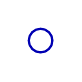
\begin{tikzpicture}[baseline=-0.5ex]
  \draw[thick, blue!70!black] (0,0) circle (0.15);
\end{tikzpicture}
& Compliance expansion zone & Strain reservoir \\[6pt]


\begin{tikzpicture}[baseline=-0.5ex]
  \draw[thick, red!70!black, ->] (0.15,0) arc (0:300:0.15);
\end{tikzpicture}
& Chiral rotation (TRS breaking) & Circulator \\[6pt]

\begin{tikzpicture}[baseline=-0.5ex]
  \draw[thick, purple!80!black] (0,0) node {$\infty$};
\end{tikzpicture}
& Topological winding number ($Q=1$) & Soliton trap \\[6pt]

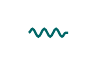
\begin{tikzpicture}[baseline=-0.5ex]
  \draw[thick, teal!80!black, decorate, decoration={snake, amplitude=0.5mm, segment length=1.5mm}] (-0.25,0) -- (0.25,0);
\end{tikzpicture}
& Phase velocity retardation & Corrugated delay line \\[6pt]


\begin{tikzpicture}[baseline=-0.5ex]
  \draw[thick, orange!80!black] (0,-0.15) -- (0.25, 0.0) -- (0, 0.15);
\end{tikzpicture}
& Continuous impedance gradient & Klopfenstein taper, Diode funnel \\[6pt]


\begin{tikzpicture}[baseline=-0.5ex]
  \draw[ultra thick, red!60!black] (0,-0.18) -- (0, 0.18);
\end{tikzpicture}
& Total reflection boundary ($\Gamma=1$) & Soliton mirrors, Fabry-Perot cavity \\[6pt]

\bottomrule
\end{tabular}
\caption{The seven canonical VCA schematic markers.}
\label{tab:vca_markers}
\end{table}

\newpage

\section{Canonical Symbol Catalogue}

%% ============================================================
%% 1. GEOMETRIC DIODE
%% ============================================================
\subsection{Geometric Diode (Asymmetric Funnel)}
\label{sym:geometric_diode}

\begin{figure}[ht]
\centering
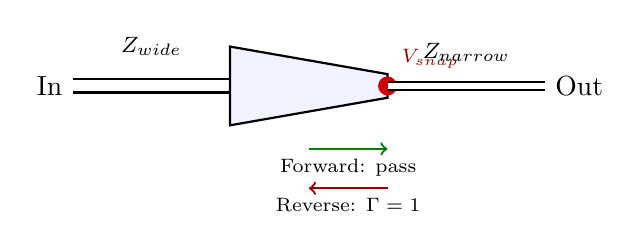
\begin{tikzpicture}[scale=1.0, thick]

  % -- Input waveguide (wide) --
  \draw[double, double distance=4pt] (-3.5, 0) -- (-1.5, 0);
  \node[above] at (-2.5, 0.25) {\footnotesize $Z_{wide}$};

  % -- Taper body --
  \draw[fill=blue!5, draw=black] (-1.5, 0.5) -- (0.5, 0.15) -- (0.5, -0.15) -- (-1.5, -0.5) -- cycle;

  % -- Saturation point --
  \fill[red!80!black] (0.5, 0) circle (0.12);
  \node[above right, font=\scriptsize, red!60!black] at (0.55, 0.1) {$V_{snap}$};

  % -- Output waveguide (narrow) --
  \draw[double, double distance=2pt] (0.5, 0) -- (2.5, 0);
  \node[above] at (1.5, 0.18) {\footnotesize $Z_{narrow}$};

  % -- Port labels --
  \node[left] at (-3.5, 0) {In};
  \node[right] at (2.5, 0) {Out};

  % -- Forward arrow --
  \draw[->, thick, green!50!black] (-0.5, -0.8) -- (0.5, -0.8);
  \node[below, font=\scriptsize] at (0, -0.8) {Forward: pass};

  % -- Reverse arrow --
  \draw[->, thick, red!60!black] (0.5, -1.3) -- (-0.5, -1.3);
  \node[below, font=\scriptsize] at (0, -1.3) {Reverse: $\Gamma = 1$};

\end{tikzpicture}
\caption{\textbf{Geometric Diode.} The tapered waveguide funnels forward waves through a smooth impedance gradient ($Z_{wide} \to Z_{narrow}$). Reverse waves compress into the narrow choke, exceeding the Axiom 4 saturation threshold $V_{snap}$ and reflecting totally. The filled dot ({\color{red!80!black}$\bullet$}) marks the saturation boundary.}
\label{fig:sym_diode}
\end{figure}

\noindent\textit{EE Equivalent:} P-N Junction Diode. \quad\textit{Key Parameter:} $V_{snap} = m_e c^2 / e \approx 511\text{ kV}$.

%% ============================================================
%% 2. GEOMETRIC TRIODE
%% ============================================================
\subsection{Geometric Triode (Transverse Saturation Throttle)}
\label{sym:geometric_triode}

\begin{figure}[ht]
\centering
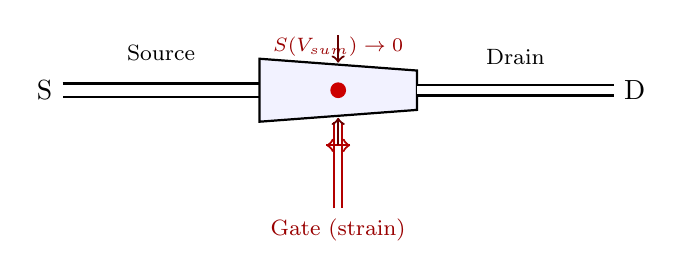
\begin{tikzpicture}[scale=1.0, thick]

  % -- Source waveguide --
  \draw[double, double distance=4pt] (-3.5, 0) -- (-1.0, 0);
  \node[above] at (-2.25, 0.25) {\footnotesize Source};

  % -- Channel body (variable width) --
  \draw[fill=blue!5, draw=black] (-1.0, 0.4) -- (1.0, 0.25) -- (1.0, -0.25) -- (-1.0, -0.4) -- cycle;

  % -- Drain waveguide --
  \draw[double, double distance=3pt] (1.0, 0) -- (3.5, 0);
  \node[above] at (2.25, 0.2) {\footnotesize Drain};

  % -- Gate (transverse strain) --
  \draw[double, double distance=2pt, red!70!black] (0, -1.5) -- (0, -0.4);
  \draw[->, red!70!black, thick] (-0.15, -0.7) -- (0.15, -0.7);
  \draw[->, red!70!black, thick] (0.15, -0.7) -- (-0.15, -0.7);
  \node[below, font=\footnotesize, red!60!black] at (0, -1.5) {Gate (strain)};

  % -- Saturation zone --
  \fill[red!80!black] (0, 0) circle (0.1);
  \node[above, font=\scriptsize, red!60!black] at (0, 0.3) {$S(V_{sum}) \to 0$};

  % -- Squeeze arrows --
  \draw[->, thick, red!40!black] (0, 0.7) -- (0, 0.35);
  \draw[->, thick, red!40!black] (0, -0.7) -- (0, -0.35);

  % Port labels
  \node[left] at (-3.5, 0) {S};
  \node[right] at (3.5, 0) {D};

\end{tikzpicture}
\caption{\textbf{Geometric Triode.} The transverse gate waveguide applies strain orthogonal to the longitudinal Source--Drain channel, physically squeezing the effective channel width. At the intersection ({\color{red!80!black}$\bullet$}), the total field $V_{sum} = \sqrt{V_{lon}^2 + V_{tr}^2}$ approaches $V_{snap}$, driving impedance $Z_{eff} \to \infty$ and blocking forward propagation. Arrows indicate the squeeze direction.}
\label{fig:sym_triode}
\end{figure}

\noindent\textit{EE Equivalent:} MOSFET / FET. \quad\textit{Key Equation:} $S(V) = \sqrt{1-(V_{sum}/V_{snap})^2}$.

%% ============================================================
%% 3. STRAIN RESERVOIR
%% ============================================================
\subsection{Strain Reservoir (Topological Capacitance)}
\label{sym:strain_reservoir}

\begin{figure}[ht]
\centering
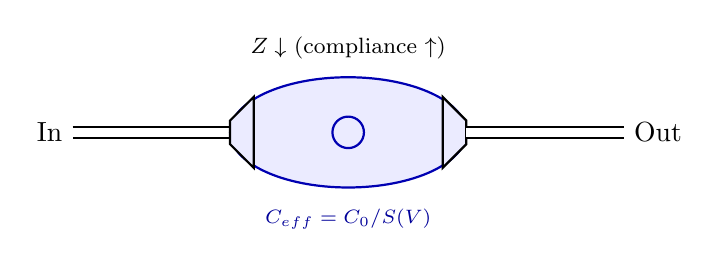
\begin{tikzpicture}[scale=1.0, thick]

  % -- Input waveguide --
  \draw[double, double distance=3pt] (-3.5, 0) -- (-1.5, 0);

  % -- Cavity (expanded compliance) --
  \draw[fill=blue!8, draw=blue!70!black, thick] (0, 0) ellipse (1.5 and 0.7);
  \draw[blue!70!black, thick] (0, 0) circle (0.2);
  \node[font=\scriptsize, blue!60!black] at (0, -1.1) {$C_{eff} = C_0 / S(V)$};

  % -- Input neck taper --
  \draw[fill=blue!8, draw=black] (-1.5, 0.15) -- (-1.5, -0.15) -- (-1.2, -0.45) -- (-1.2, 0.45) -- cycle;

  % -- Output neck taper --
  \draw[fill=blue!8, draw=black] (1.2, 0.45) -- (1.2, -0.45) -- (1.5, -0.15) -- (1.5, 0.15) -- cycle;

  % -- Output waveguide --
  \draw[double, double distance=3pt] (1.5, 0) -- (3.5, 0);

  % -- Impedance label --
  \node[above] at (0, 0.8) {\footnotesize $Z \downarrow$ (compliance $\uparrow$)};

  % Port labels
  \node[left] at (-3.5, 0) {In};
  \node[right] at (3.5, 0) {Out};

\end{tikzpicture}
\caption{\textbf{Strain Reservoir.} An expanded cavity in the waveguide locally plummets impedance $Z_0 \propto \sqrt{L/C}$ via massive compliance multiplication. The inner ring ({\color{blue!70!black}$\circ$}) marks the compliance expansion zone. Energy is stored as tensioned space volumetrically within the Axiom 4 yield limit.}
\label{fig:sym_reservoir}
\end{figure}

\noindent\textit{EE Equivalent:} Capacitor. \quad\textit{Key Physics:} $U_{strain} \propto \int (1-S(V))\,dx$.

%% ============================================================
%% 4. SOLITON KINK TRAP
%% ============================================================
\subsection{Soliton Kink Trap (Non-Volatile Memory)}
\label{sym:soliton_trap}

\begin{figure}[ht]
\centering
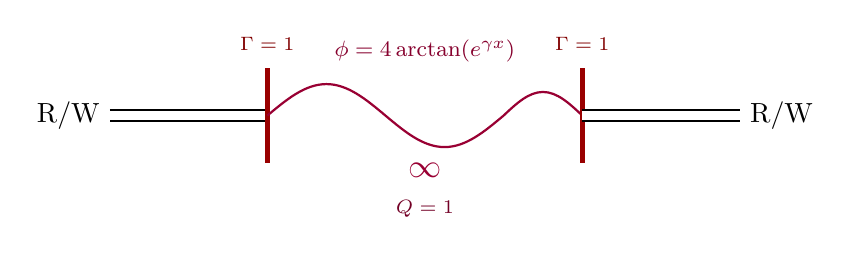
\begin{tikzpicture}[scale=1.0, thick]

  % -- Input waveguide --
  \draw[double, double distance=3pt] (-4.0, 0) -- (-2.0, 0);

  % -- Left mirror --
  \draw[ultra thick, red!60!black] (-2.0, -0.6) -- (-2.0, 0.6);
  \node[above, font=\scriptsize, red!50!black] at (-2.0, 0.7) {$\Gamma = 1$};

  % -- Cavity with knot (Q=1 state) --
  \draw[thick, purple!80!black, smooth] (-2.0, 0) sin (-1.25, 0.4) cos (-0.5, 0) sin (0.25, -0.4) cos (1.0, 0) sin (1.5, 0.3) cos (2.0, 0);
  \node[above, font=\footnotesize, purple!70!black] at (0, 0.55) {$\phi = 4\arctan(e^{\gamma x})$};

  % -- Winding number indicator --
  \node[font=\large, purple!80!black] at (0, -0.7) {$\infty$};
  \node[below, font=\scriptsize, purple!60!black] at (0, -0.95) {$Q = 1$};

  % -- Right mirror --
  \draw[ultra thick, red!60!black] (2.0, -0.6) -- (2.0, 0.6);
  \node[above, font=\scriptsize, red!50!black] at (2.0, 0.7) {$\Gamma = 1$};

  % -- Output waveguide --
  \draw[double, double distance=3pt] (2.0, 0) -- (4.0, 0);

  % Port labels
  \node[left] at (-4.0, 0) {R/W};
  \node[right] at (4.0, 0) {R/W};

\end{tikzpicture}
\caption{\textbf{Soliton Kink Trap ($Q=1$).} Two total-reflection mirrors ({\color{red!60!black}$\mid$}, $\Gamma = 1$) confine a sine-Gordon soliton. The {\color{purple!80!black}$\infty$} symbol indicates the topological winding number. With no knot ($Q=0$), the interior is empty. Zero standby power; state persists indefinitely until deliberately ruptured.}
\label{fig:sym_soliton}
\end{figure}

\noindent\textit{EE Equivalent:} Flash / NAND Memory. \quad\textit{Key Equation:} $\phi(x) = 4\arctan(e^{\gamma(x-vt)})$.

%% ============================================================
%% 5. DIELECTRIC CORRUGATION (DELAY LINE)
%% ============================================================
\subsection{Dielectric Corrugation (Slow-Wave Delay)}
\label{sym:delay_line}

\begin{figure}[ht]
\centering
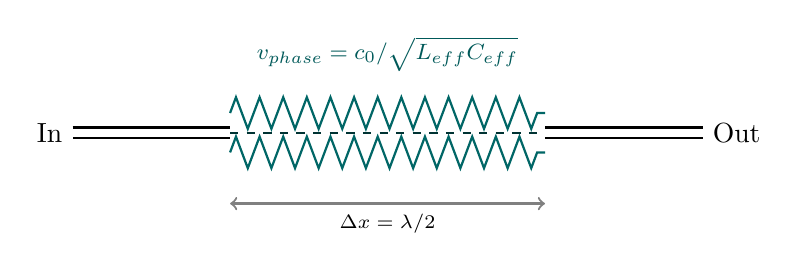
\begin{tikzpicture}[scale=1.0, thick]

  % -- Input waveguide --
  \draw[double, double distance=3pt] (-4.0, 0) -- (-2.0, 0);

  % -- Corrugated section (top wall) --
  \draw[thick, teal!80!black, decorate, decoration={zigzag, amplitude=2mm, segment length=3mm}] (-2.0, 0.25) -- (2.0, 0.25);

  % -- Corrugated section (bottom wall) --
  \draw[thick, teal!80!black, decorate, decoration={zigzag, amplitude=2mm, segment length=3mm}] (-2.0, -0.25) -- (2.0, -0.25);

  % -- Center line (wave path) --
  \draw[thick, teal!40!black, dashed] (-2.0, 0) -- (2.0, 0);

  % -- Slow-wave annotation --
  \node[above, font=\footnotesize, teal!70!black] at (0, 0.65) {$v_{phase} = c_0 / \sqrt{L_{eff}C_{eff}}$};

  % -- Delay markers --
  \draw[<->, thick, gray] (-2.0, -0.9) -- (2.0, -0.9);
  \node[below, font=\scriptsize] at (0, -0.9) {$\Delta x = \lambda / 2$};

  % -- Output waveguide --
  \draw[double, double distance=3pt] (2.0, 0) -- (4.0, 0);

  % Port labels
  \node[left] at (-4.0, 0) {In};
  \node[right] at (4.0, 0) {Out};

\end{tikzpicture}
\caption{\textbf{Dielectric Corrugation.} The corrugated waveguide walls ({\color{teal!80!black}$\approx$}) stretch the effective surface path, raising local $L_{eff}$ and $C_{eff}$ symmetrically. Phase velocity is reduced without scattering the waveform. Impedance $Z_0$ is preserved because $L$ and $C$ scale together.}
\label{fig:sym_delay}
\end{figure}

\noindent\textit{EE Equivalent:} RC Delay / Transmission Line Stub. \quad\textit{Key Physics:} Lossless; $Z_0 = \sqrt{L_{eff}/C_{eff}}$ constant.

%% ============================================================
%% 6. TOPOLOGICAL Y-JUNCTION (XOR)
%% ============================================================
\subsection{Topological Y-Junction (XOR Logic)}
\label{sym:y_junction}

\begin{figure}[ht]
\centering
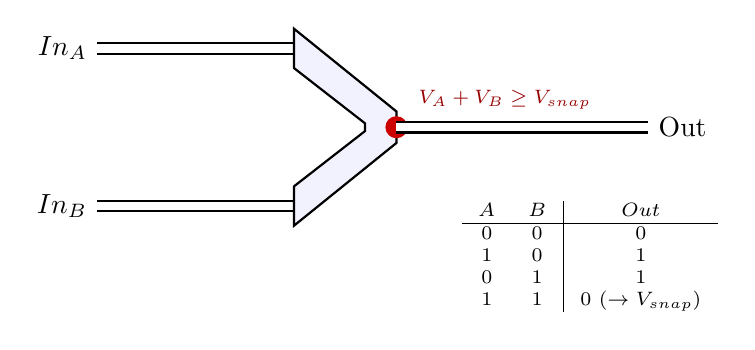
\begin{tikzpicture}[scale=1.0, thick]

  % -- Input A waveguide --
  \draw[double, double distance=3pt] (-4.0, 1.0) -- (-1.5, 1.0);
  \node[left] at (-4.0, 1.0) {$In_A$};

  % -- Input B waveguide --
  \draw[double, double distance=3pt] (-4.0, -1.0) -- (-1.5, -1.0);
  \node[left] at (-4.0, -1.0) {$In_B$};

  % -- Merge tapers --
  \draw[fill=blue!5, draw=black] (-1.5, 1.25) -- (-0.2, 0.2) -- (-0.2, -0.2) -- (-1.5, -1.25) -- (-1.5, -0.75) -- (-0.6, -0.05) -- (-0.6, 0.05) -- (-1.5, 0.75) -- cycle;

  % -- Saturation zone --
  \fill[red!80!black] (-0.2, 0) circle (0.14);
  \node[above right, font=\scriptsize, red!60!black] at (-0.05, 0.1) {$V_A + V_B \geq V_{snap}$};

  % -- Output waveguide --
  \draw[double, double distance=3pt] (-0.2, 0) -- (3.0, 0);
  \node[right] at (3.0, 0) {Out};

  % -- Truth table --
  \node[font=\scriptsize, anchor=north west] at (0.5, -0.8) {
    \begin{tabular}{cc|c}
    $A$ & $B$ & $Out$ \\ \hline
    0 & 0 & 0 \\
    1 & 0 & 1 \\
    0 & 1 & 1 \\
    1 & 1 & 0\ ($\to V_{snap}$)
    \end{tabular}
  };

\end{tikzpicture}
\caption{\textbf{Topological Y-Junction (XOR).} Two waveguides merge at a choke point. When both inputs fire simultaneously, their constructive superposition drives the junction field past the saturation threshold $V_{snap}$, collapsing transmission ($S \to 0$). Single-input waves pass unimpeded. The filled dot ({\color{red!80!black}$\bullet$}) marks the nonlinear saturation zone.}
\label{fig:sym_xor}
\end{figure}

\noindent\textit{EE Equivalent:} XOR Gate (CMOS). \quad\textit{Key Physics:} $S(V) \to 0$ when $V_{sum} \geq V_{snap}$.

%% ============================================================
%% 7. CHIRAL CIRCULATOR
%% ============================================================
\subsection{Chiral Wave Circulator (3-Port Router)}
\label{sym:circulator}

\begin{figure}[ht]
\centering
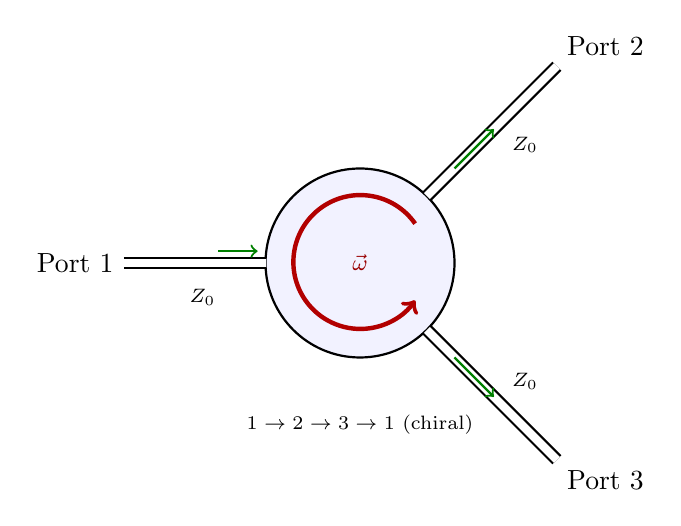
\begin{tikzpicture}[scale=1.0, thick]

  % -- Central vortex body --
  \draw[fill=blue!5, draw=black, thick] (0,0) circle (1.2);

  % -- Rotation arrow --
  \draw[ultra thick, red!70!black, ->] (0.7, 0.5) arc (35:325:0.85);
  \node[font=\footnotesize, red!60!black] at (0, 0) {$\vec{\omega}$};

  % -- Port 1 (left) --
  \draw[double, double distance=3pt] (-3.0, 0) -- (-1.2, 0);
  \node[left] at (-3.0, 0) {Port 1};

  % -- Port 2 (top-right) --
  \draw[double, double distance=3pt] (0.85, 0.85) -- (2.5, 2.5);
  \node[above right] at (2.5, 2.5) {Port 2};

  % -- Port 3 (bottom-right) --
  \draw[double, double distance=3pt] (0.85, -0.85) -- (2.5, -2.5);
  \node[below right] at (2.5, -2.5) {Port 3};

  % -- Z_0 annotations --
  \node[below, font=\scriptsize] at (-2.0, -0.2) {$Z_0$};
  \node[right, font=\scriptsize] at (1.8, 1.5) {$Z_0$};
  \node[right, font=\scriptsize] at (1.8, -1.5) {$Z_0$};

  % -- Flow arrows --
  \draw[->, thick, green!50!black] (-1.8, 0.15) -- (-1.3, 0.15);
  \draw[->, thick, green!50!black] (1.2, 1.2) -- (1.7, 1.7);
  \draw[->, thick, green!50!black] (1.2, -1.2) -- (1.7, -1.7);

  % -- Routing annotation --
  \node[below, font=\scriptsize] at (0, -1.8) {$1 \to 2 \to 3 \to 1$ (chiral)};

\end{tikzpicture}
\caption{\textbf{Chiral Wave Circulator.} A metric Faraday vortex ({\color{red!70!black}$\circlearrowleft$}) inside the central body breaks time-reversal symmetry, routing waves $1 \to 2 \to 3 \to 1$ circularly. All three ports are impedance-matched to $Z_0 = 376.73\,\Omega$, ensuring zero return loss. This is the VCA equivalent of an RF ferrite circulator.}
\label{fig:sym_circulator}
\end{figure}

\noindent\textit{EE Equivalent:} RF Ferrite Circulator. \quad\textit{Key Parameter:} $Z_0 = \sqrt{\mu_0/\epsilon_0} \approx 376.73\,\Omega$.

%% ============================================================
%% 8. THERMAL BAFFLE
%% ============================================================
\subsection{Thermal Baffle (Entropy Decay Sink)}
\label{sym:thermal_baffle}

\begin{figure}[ht]
\centering
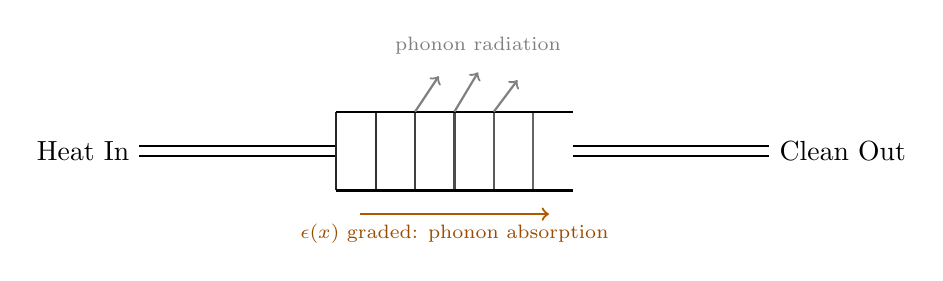
\begin{tikzpicture}[scale=1.0, thick]

  % -- Input waveguide --
  \draw[double, double distance=3pt] (-4.0, 0) -- (-1.5, 0);
  \node[left] at (-4.0, 0) {Heat In};

  % -- Graded permittivity body --
  \draw[gray!30!black, thick] (-1.5, -0.5) -- (-1.5, 0.5);
  \draw[gray!40!black, thick] (-1.0, -0.5) -- (-1.0, 0.5);
  \draw[gray!50!black, thick] (-0.5, -0.5) -- (-0.5, 0.5);
  \draw[gray!60!black, thick] (0, -0.5) -- (0, 0.5);
  \draw[gray!70!black, thick] (0.5, -0.5) -- (0.5, 0.5);
  \draw[gray!80!black, thick] (1.0, -0.5) -- (1.0, 0.5);
  \draw[thick] (-1.5, 0.5) -- (1.5, 0.5);
  \draw[thick] (-1.5, -0.5) -- (1.5, -0.5);

  % -- Fade annotation --
  \draw[->, thick, orange!70!black] (-1.2, -0.8) -- (1.2, -0.8);
  \node[below, font=\scriptsize, orange!60!black] at (0, -0.8) {$\epsilon(x)$ graded: phonon absorption};

  % -- Scattered phonon arrows --
  \draw[->, gray, thick] (0, 0.5) -- (0.3, 1.0);
  \draw[->, gray, thick] (0.5, 0.5) -- (0.8, 0.9);
  \draw[->, gray, thick] (-0.5, 0.5) -- (-0.2, 0.95);
  \node[above, font=\scriptsize, gray] at (0.3, 1.1) {phonon radiation};

  % -- Output waveguide (cleaned) --
  \draw[double, double distance=3pt] (1.5, 0) -- (4.0, 0);
  \node[right] at (4.0, 0) {Clean Out};

\end{tikzpicture}
\caption{\textbf{Thermal Baffle.} Graded permittivity trenches progressively absorb chaotic phonon energy (scattered arrows), converting computational entropy into isotropic lattice drag. The vertical lines darken with depth, indicating increasing absorption. Signal exits cleaned of stochastic noise.}
\label{fig:sym_baffle}
\end{figure}

\noindent\textit{EE Equivalent:} Heat Sink / Decoupling Network. \quad\textit{Key Physics:} Landauer entropy $\Delta Q \geq kT\ln 2$ radiated as phonons.

%% ============================================================
%% 9. KLOPFENSTEIN TAPER (ROUTING)
%% ============================================================
\subsection{Klopfenstein Taper (Phase-Locked Routing)}
\label{sym:klopfenstein}

\begin{figure}[ht]
\centering
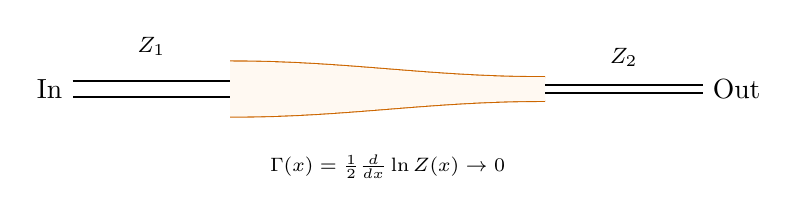
\begin{tikzpicture}[scale=1.0, thick]

  % -- Wide waveguide --
  \draw[double, double distance=5pt] (-4.0, 0) -- (-2.0, 0);
  \node[above] at (-3.0, 0.3) {\footnotesize $Z_1$};

  % -- Taper body (smooth exponential curve) --
  \draw[thick, orange!80!black] (-2.0, 0.35) .. controls (-0.5, 0.35) and (0.5, 0.15) .. (2.0, 0.15);
  \draw[thick, orange!80!black] (-2.0, -0.35) .. controls (-0.5, -0.35) and (0.5, -0.15) .. (2.0, -0.15);

  % -- Fill --
  \fill[orange!5] (-2.0, 0.35) .. controls (-0.5, 0.35) and (0.5, 0.15) .. (2.0, 0.15) -- (2.0, -0.15) .. controls (0.5, -0.15) and (-0.5, -0.35) .. (-2.0, -0.35) -- cycle;

  % -- Narrow waveguide --
  \draw[double, double distance=2pt] (2.0, 0) -- (4.0, 0);
  \node[above] at (3.0, 0.15) {\footnotesize $Z_2$};

  % -- Reflection coefficient --
  \node[below, font=\scriptsize] at (0, -0.7) {$\Gamma(x) = \frac{1}{2}\frac{d}{dx}\ln Z(x) \to 0$};

  % Port labels
  \node[left] at (-4.0, 0) {In};
  \node[right] at (4.0, 0) {Out};

\end{tikzpicture}
\caption{\textbf{Klopfenstein Taper.} The smooth exponential impedance gradient ({\color{orange!80!black}taper lines}) transitions $Z_1 \to Z_2$ with zero return loss ($\Gamma = 0$). This replaces all discrete right-angle PCB traces in VCA layouts, eliminating parasitic reflections and standing-wave heat generation. The waveguide width encodes impedance directly.}
\label{fig:sym_klopfenstein}
\end{figure}

\noindent\textit{EE Equivalent:} Impedance Matching / Transformer. \quad\textit{Key Equation:} $\Gamma(x) = \frac{1}{2}\frac{d}{dx}\ln Z(x)$.

%% ============================================================
%% 10. TOPOLOGICAL RING OSCILLATOR
%% ============================================================
\subsection{Topological Ring Oscillator (Native Clock)}
\label{sym:ring_oscillator}

\begin{figure}[ht]
\centering
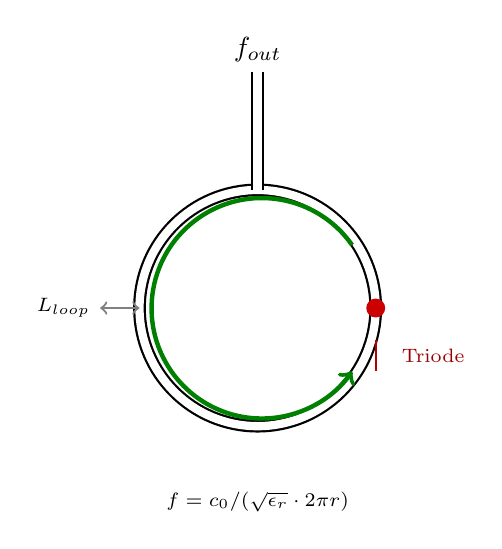
\begin{tikzpicture}[scale=1.0, thick]

  % -- Ring body --
  \draw[double, double distance=3pt] (0, 0) circle (1.5);

  % -- Circulation arrow --
  \draw[->, ultra thick, green!50!black] (1.2, 0.8) arc (35:325:1.4);

  % -- Triode inverter (notch) --
  \fill[red!80!black] (1.5, 0) circle (0.12);
  \draw[thick, red!70!black] (1.5, -0.4) -- (1.5, -0.8);
  \node[right, font=\scriptsize, red!60!black] at (1.7, -0.6) {Triode};

  % -- Output tap --
  \draw[double, double distance=3pt] (0, 1.5) -- (0, 3.0);
  \node[above] at (0, 3.0) {$f_{out}$};

  % -- Frequency annotation --
  \node[below, font=\scriptsize] at (0, -2.2) {$f = c_0 / (\sqrt{\epsilon_r} \cdot 2\pi r)$};

  % -- Loop length --
  \draw[<->, thick, gray] (-2.0, 0) -- (-1.5, 0);
  \node[left, font=\scriptsize] at (-2.0, 0) {$L_{loop}$};

\end{tikzpicture}
\caption{\textbf{Topological Ring Oscillator.} A closed-loop waveguide with a single Geometric Triode inverter ({\color{red!80!black}$\bullet$}) generates native self-sustaining oscillation. The frequency is set purely by the geometric loop circumference and substrate permittivity. No external crystal or PLL is required.}
\label{fig:sym_ring_osc}
\end{figure}

\noindent\textit{EE Equivalent:} Quartz Crystal Oscillator / PLL. \quad\textit{Key Physics:} $f = c_0 / (\sqrt{\epsilon_r} \cdot 2L_{loop})$.

%% ============================================================
%% 11. COANDA AMPLIFIER
%% ============================================================
\subsection{Coanda Amplifier (Fluidic Boundary Steering)}
\label{sym:coanda}

\begin{figure}[ht]
\centering
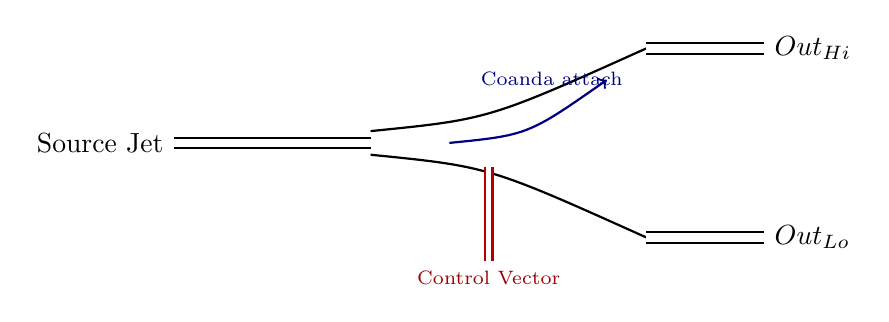
\begin{tikzpicture}[scale=1.0, thick]

  % -- Source jet waveguide --
  \draw[double, double distance=3pt] (-4.0, 0) -- (-1.5, 0);
  \node[left] at (-4.0, 0) {Source Jet};

  % -- Diverging body --
  \draw[thick] (-1.5, 0.15) .. controls (0, 0.3) .. (2.0, 1.2);
  \draw[thick] (-1.5, -0.15) .. controls (0, -0.3) .. (2.0, -1.2);

  % -- Output Hi --
  \draw[double, double distance=3pt] (2.0, 1.2) -- (3.5, 1.2);
  \node[right] at (3.5, 1.2) {$Out_{Hi}$};

  % -- Output Lo --
  \draw[double, double distance=3pt] (2.0, -1.2) -- (3.5, -1.2);
  \node[right] at (3.5, -1.2) {$Out_{Lo}$};

  % -- Control port (transverse) --
  \draw[double, double distance=2pt, red!70!black] (0, -1.5) -- (0, -0.3);
  \node[below, font=\scriptsize, red!60!black] at (0, -1.5) {Control Vector};

  % -- Coanda attachment annotation --
  \draw[->, thick, blue!50!black] (-0.5, 0) .. controls (0.5, 0.1) .. (1.5, 0.8);
  \node[above, font=\scriptsize, blue!50!black] at (0.8, 0.6) {Coanda attach};

\end{tikzpicture}
\caption{\textbf{Coanda Amplifier.} A high-velocity source jet enters a diverging cavity. The Coanda effect causes the jet to lock onto one wall ({\color{blue!50!black}curved arrow}). A small transverse control signal deflects the attachment point, switching the output between $Out_{Hi}$ and $Out_{Lo}$ with massive gain. Zero friction; purely spatial momentum steering.}
\label{fig:sym_coanda}
\end{figure}

\noindent\textit{EE Equivalent:} Operational Amplifier (high-gain). \quad\textit{Key Physics:} Frictionless jet deflection, no $kT$ barrier.

%% ============================================================
%% 12. AXIOMATIC TRANSDUCER
%% ============================================================
\subsection{Axiomatic Transducer (VCA $\leftrightarrow$ Legacy Bridge)}
\label{sym:transducer}

\begin{figure}[ht]
\centering
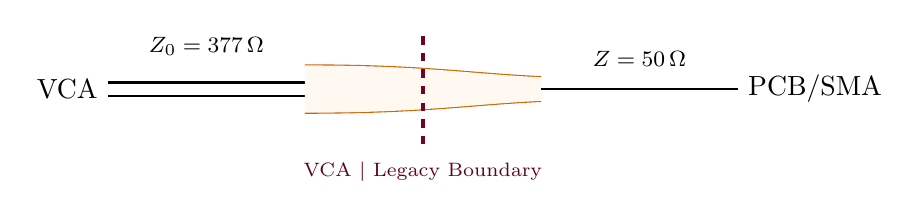
\begin{tikzpicture}[scale=1.0, thick]

  % -- VCA side (double line, Z_0) --
  \draw[double, double distance=4pt] (-4.0, 0) -- (-1.5, 0);
  \node[above] at (-2.75, 0.3) {\footnotesize $Z_0 = 377\,\Omega$};

  % -- Taper body (Klopfenstein VCA->50ohm) --
  \draw[thick, orange!80!black] (-1.5, 0.3) .. controls (0, 0.3) and (0.5, 0.2) .. (1.5, 0.15);
  \draw[thick, orange!80!black] (-1.5, -0.3) .. controls (0, -0.3) and (0.5, -0.2) .. (1.5, -0.15);
  \fill[orange!5] (-1.5, 0.3) .. controls (0, 0.3) and (0.5, 0.2) .. (1.5, 0.15) -- (1.5, -0.15) .. controls (0.5, -0.2) and (0, -0.3) .. (-1.5, -0.3) -- cycle;

  % -- Boundary marker --
  \draw[ultra thick, purple!60!black, dashed] (0, -0.7) -- (0, 0.7);
  \node[below, font=\scriptsize, purple!50!black] at (0, -0.8) {VCA $\mid$ Legacy Boundary};

  % -- Legacy side (single line, 50ohm) --
  \draw[thick] (1.5, 0) -- (4.0, 0);
  \node[above] at (2.75, 0.15) {\footnotesize $Z = 50\,\Omega$};

  % Port labels
  \node[left] at (-4.0, 0) {VCA};
  \node[right] at (4.0, 0) {PCB/SMA};

\end{tikzpicture}
\caption{\textbf{Axiomatic Transducer.} A continuous Klopfenstein impedance taper bridges the vacuum domain ($Z_0 = 377\,\Omega$, double-line waveguide) to legacy $50\,\Omega$ systems (single-line trace). The dashed boundary marks the transition from axiomatic to conventional electronics. Zero insertion loss when the taper length $\geq \lambda/2$.}
\label{fig:sym_transducer}
\end{figure}

\noindent\textit{EE Equivalent:} SMA Connector / Balun. \quad\textit{Key Physics:} $\Gamma = 0$ continuous matching from $377\,\Omega$ to $50\,\Omega$.

%% ============================================================
%% 13. GEOMETRIC TESLA VALVE
%% ============================================================
\subsection{Geometric Tesla Valve (Axiomatic Rectifier)}
\label{sym:tesla_valve}

\begin{figure}[ht]
\centering
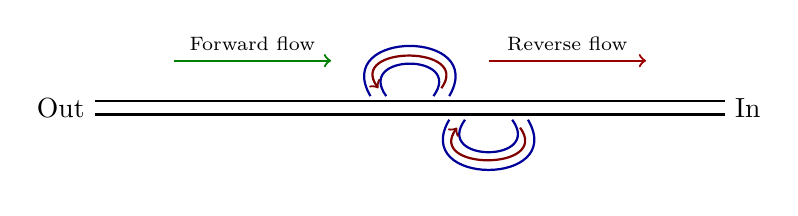
\begin{tikzpicture}[scale=1.0, thick]

  % -- Main channel --
  \draw[double, double distance=4pt] (-4.0, 0) -- (4.0, 0);
  
  % -- Teardrop loop 1 (top) --
  \draw[thick, blue!60!black] (0.5, 0.15) .. controls (1.0, 1.0) and (-1.0, 1.0) .. (-0.5, 0.15);
  \draw[thick, blue!60!black] (0.3, 0.15) .. controls (0.7, 0.7) and (-0.7, 0.7) .. (-0.3, 0.15);
  
  % -- Teardrop loop 2 (bottom) --
  \draw[thick, blue!60!black] (1.5, -0.15) .. controls (2.0, -1.0) and (0.0, -1.0) .. (0.5, -0.15);
  \draw[thick, blue!60!black] (1.3, -0.15) .. controls (1.7, -0.7) and (0.3, -0.7) .. (0.7, -0.15);

  % -- Forward flow (unimpeded) --
  \draw[->, thick, green!50!black] (-3.0, 0.6) -- (-1.0, 0.6);
  \node[above, font=\scriptsize] at (-2.0, 0.6) {Forward flow};

  % -- Reverse flow (interfering) --
  \draw[<-, thick, red!60!black] (3.0, 0.6) -- (1.0, 0.6);
  \node[above, font=\scriptsize] at (2.0, 0.6) {Reverse flow};
  \draw[->, thick, red!50!black] (0.4, 0.25) .. controls (0.8, 0.8) and (-0.8, 0.8) .. (-0.4, 0.25);
  \draw[->, thick, red!50!black] (1.4, -0.25) .. controls (1.8, -0.8) and (0.2, -0.8) .. (0.6, -0.25);

  % -- Labels --
  \node[left] at (-4.0, 0) {Out};
  \node[right] at (4.0, 0) {In};

\end{tikzpicture}
\caption{\textbf{Geometric Tesla Valve.} A pure geometric wave rectifier. Forward waves pass mostly unimpeded along the central axis. Reverse waves are continually scooped into the recursive teardrop side-channels, wrapping around to destructively interfere with the main reverse flow. Unlike the Geometric Diode, the Tesla Valve operates completely in the linear regime (no Axiom 4 saturation dot).}
\label{fig:sym_tesla_valve}
\end{figure}

\noindent\textit{EE Equivalent:} RF Choke / Directional Coupler / Acoustic Baffle. \quad\textit{Key Physics:} Destructive path-length interference, passive rectification.

%% ============================================================
%% 14. FABRY-PEROT RESONANCE CAVITY
%% ============================================================
\subsection{Fabry-Perot Resonance Cavity}
\label{sym:resonance_cavity}

\begin{figure}[ht]
\centering
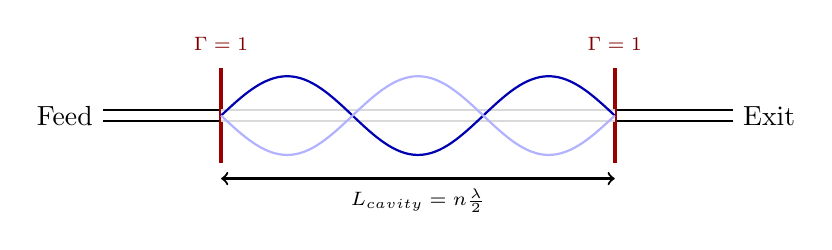
\begin{tikzpicture}[scale=1.0, thick]

  % -- External guides --
  \draw[double, double distance=3pt] (-4.0, 0) -- (-2.5, 0);
  \draw[double, double distance=3pt] (2.5, 0) -- (4.0, 0);

  % -- Boundaries --
  \draw[ultra thick, red!60!black] (-2.5, -0.6) -- (-2.5, 0.6);
  \draw[ultra thick, red!60!black] (2.5, -0.6) -- (2.5, 0.6);
  \node[above, font=\scriptsize, red!50!black] at (-2.5, 0.7) {$\Gamma = 1$};
  \node[above, font=\scriptsize, red!50!black] at (2.5, 0.7) {$\Gamma = 1$};

  % -- Internal Cavity --
  \draw[double, double distance=3pt, gray!30] (-2.5, 0) -- (2.5, 0);

  % -- Standing wave --
  \draw[thick, blue!70!black, smooth] (-2.5, 0) sin (-1.66, 0.5) cos (-0.83, 0) sin (0, -0.5) cos (0.83, 0) sin (1.66, 0.5) cos (2.5, 0);
  \draw[thick, blue!30, smooth] (-2.5, 0) sin (-1.66, -0.5) cos (-0.83, 0) sin (0, 0.5) cos (0.83, 0) sin (1.66, -0.5) cos (2.5, 0);

  % -- Cavity length annotation --
  \draw[<->, thick] (-2.5, -0.8) -- (2.5, -0.8);
  \node[below, font=\scriptsize] at (0, -0.8) {$L_{cavity} = n\frac{\lambda}{2}$};

  % -- Labels --
  \node[left] at (-4.0, 0) {Feed};
  \node[right] at (4.0, 0) {Exit};

\end{tikzpicture}
\caption{\textbf{Resonance Cavity.} Two extreme impedance step-boundaries ({\color{red!60!black}$\mid$}) form an isolated chamber where sequential waves superimpose. When the length is an integer multiple of $\lambda/2$, massive constructive interference builds a native standing wave (blue envelope). This structure acts as a passive wave accumulator or high-$Q$ filter.}
\label{fig:sym_resonance_cavity}
\end{figure}

\noindent\textit{EE Equivalent:} LC Tank / Cavity Resonator. \quad\textit{Key Physics:} $f_{res} = n \cdot c_0 / (2L_{cavity})$.

%% ============================================================
%% 15. TENSOR PLATE ALU
%% ============================================================
\subsection{Tensor Plate ALU (Refractive Computing)}
\label{sym:tensor_plate}

\begin{figure}[ht]
\centering
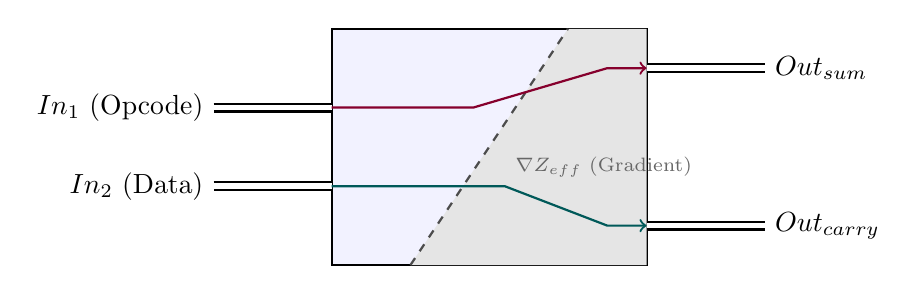
\begin{tikzpicture}[scale=1.0, thick]

  % -- Massive central chamber --
  \draw[fill=blue!5, draw=black] (-2.0, 1.5) rectangle (2.0, -1.5);
  
  % -- Graded refractive zone (angled) --
  \fill[gray!20] (-1.0, -1.5) -- (1.0, 1.5) -- (2.0, 1.5) -- (2.0, -1.5) -- cycle;
  \draw[dashed, gray!60!black] (-1.0, -1.5) -- (1.0, 1.5);
  \node[below right, font=\scriptsize, gray!80!black] at (0.2, 0) {$\nabla Z_{eff}$ (Gradient)};

  % -- Input lines --
  \draw[double, double distance=2pt] (-3.5, 0.5) -- (-2.0, 0.5);
  \draw[double, double distance=2pt] (-3.5, -0.5) -- (-2.0, -0.5);
  \node[left] at (-3.5, 0.5) {$In_1$ (Opcode)};
  \node[left] at (-3.5, -0.5) {$In_2$ (Data)};

  % -- Refracted beams --
  \draw[->, thick, purple!70!black] (-2.0, 0.5) -- (-0.2, 0.5) -- (1.5, 1.0) -- (2.0, 1.0);
  \draw[->, thick, teal!70!black] (-2.0, -0.5) -- (0.2, -0.5) -- (1.5, -1.0) -- (2.0, -1.0);

  % -- Output lines --
  \draw[double, double distance=2pt] (2.0, 1.0) -- (3.5, 1.0);
  \draw[double, double distance=2pt] (2.0, -1.0) -- (3.5, -1.0);
  \node[right] at (3.5, 1.0) {$Out_{sum}$};
  \node[right] at (3.5, -1.0) {$Out_{carry}$};

\end{tikzpicture}
\caption{\textbf{Tensor Plate ALU.} A wide 2D cavity containing a dynamically driven structural gradient ($\nabla Z_{eff}$, shaded region). Inlet waves act as parallel wavefronts that refract (bend) according to the vacuum variant of Snell's Law induced by the gradient. The spatial intersection of multiple refracted beams physically calculates logic/arithmetic matrices simultaneously.}
\label{fig:sym_tensor_plate}
\end{figure}

\noindent\textit{EE Equivalent:} Arithmetic Logic Unit / Multiplier. \quad\textit{Key Physics:} Snell's Law for metric compliance $\frac{\sin\theta_1}{\sin\theta_2} = \frac{v_{ph,1}}{v_{ph,2}}$.

%% ============================================================
%% 16. INTERFERENCE WAVE ROUTER
%% ============================================================
\subsection{Interference Wave Router (Mach-Zehnder Switch)}
\label{sym:interference_router}

\begin{figure}[ht]
\centering
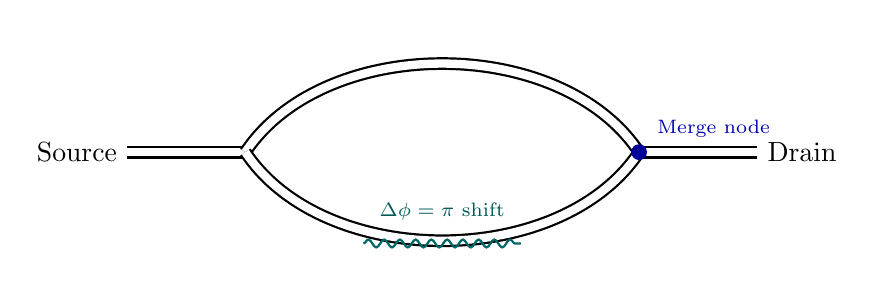
\begin{tikzpicture}[scale=1.0, thick]

  % -- Splitter input --
  \draw[double, double distance=3pt] (-4.0, 0) -- (-2.5, 0);
  \node[left] at (-4.0, 0) {Source};

  % -- Upper arm --
  \draw[double, double distance=3pt] (-2.5, 0) .. controls (-1.5, 1.5) and (1.5, 1.5) .. (2.5, 0);

  % -- Lower arm (Delay) --
  \draw[double, double distance=3pt] (-2.5, 0) .. controls (-1.5, -1.5) and (1.5, -1.5) .. (2.5, 0);
  
  % -- SWS delay corrugations on lower arm --
  \draw[thick, teal!80!black, decorate, decoration={snake, amplitude=0.5mm, segment length=2mm}] (-1.0, -1.16) -- (1.0, -1.16);
  \node[above, font=\scriptsize, teal!70!black] at (0, -1.0) {$\Delta\phi = \pi$ shift};

  % -- Recombiner output --
  \draw[double, double distance=3pt] (2.5, 0) -- (4.0, 0);
  \node[right] at (4.0, 0) {Drain};

  % -- Flow annotations --
  \fill[blue!60!black] (2.5, 0) circle (0.1);
  \node[right, font=\scriptsize, blue!70!black] at (2.6, 0.3) {Merge node};

\end{tikzpicture}
\caption{\textbf{Interference Wave Router.} A source wave splits evenly into two legs. The lower leg passes through a geometric delay line (corrugation marker), applying a precisely machined phase shift ($\Delta\phi$). When the waves merge, their phase difference dictates whether they construct (pass) or destructively annihilate (suppress), executing logic purely via path-length geometry.}
\label{fig:sym_interference_router}
\end{figure}

\noindent\textit{EE Equivalent:} Mach-Zehnder Interferometer / Phase MUX. \quad\textit{Key Physics:} $\Delta\phi = \frac{2\pi}{\lambda_{op}} (L_2^{\rm eff} - L_1)$.

%% ============================================================
%% 17. TOPOLOGICAL DAC SYNTHESIZER
%% ============================================================
\subsection{Topological DAC Synthesizer}
\label{sym:topological_dac}

\begin{figure}[ht]
\centering
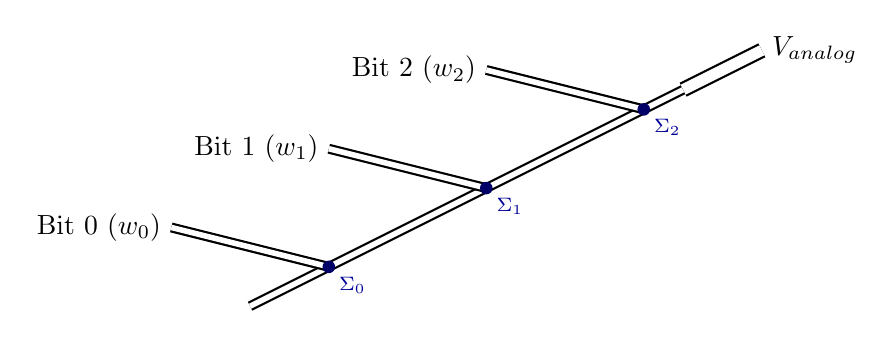
\begin{tikzpicture}[scale=1.0, thick]

  % -- Main accumulation trace --
  \draw[double, double distance=2pt] (-2.0, -1.5) -- (3.5, 1.25);
  
  % -- Bit 0 input --
  \draw[double, double distance=2pt] (-3.0, -0.5) -- (-1.0, -1.0);
  \node[left] at (-3.0, -0.5) {Bit 0 ($w_0$)};
  
  % -- Bit 1 input --
  \draw[double, double distance=2pt] (-1.0, 0.5) -- (1.0, 0.0);
  \node[left] at (-1.0, 0.5) {Bit 1 ($w_1$)};

  % -- Bit 2 input --
  \draw[double, double distance=2pt] (1.0, 1.5) -- (3.0, 1.0);
  \node[left] at (1.0, 1.5) {Bit 2 ($w_2$)};

  % -- Merging intersections --
  \fill[blue!40!black] (-1.0, -1.0) circle (0.08);
  \fill[blue!40!black] (1.0, 0.0) circle (0.08);
  \fill[blue!40!black] (3.0, 1.0) circle (0.08);

  % -- Accumulation annotations --
  \node[below right, font=\scriptsize, blue!60!black] at (-1.0, -1.0) {$\Sigma_0$};
  \node[below right, font=\scriptsize, blue!60!black] at (1.0, 0.0) {$\Sigma_1$};
  \node[below right, font=\scriptsize, blue!60!black] at (3.0, 1.0) {$\Sigma_2$};

  % -- Output --
  \draw[double, double distance=4pt] (3.5, 1.25) -- (4.5, 1.75);
  \node[right] at (4.5, 1.75) {$V_{analog}$};

\end{tikzpicture}
\caption{\textbf{Topological DAC Synthesizer.} A continuous feed-forward geometric ladder. Individual weighted "bit" waveguides inject controlled strain amplitudes sequentially into a main accumulating manifold. The final superposition wave encapsulates the analog geometric representation of the digital multi-bit vector, ready to drive complex analog features like Tensor Plates.}
\label{fig:sym_dac}
\end{figure}

\noindent\textit{EE Equivalent:} Digital-to-Analog Converter / R-2R Ladder. \quad\textit{Key Physics:} Linear superposition $V_{analog} = \sum w_i V_i$.

%% ============================================================
%% 18. CONTINUOUS FPGA MATRIX
%% ============================================================
\subsection{Continuous FPGA Matrix (Reconfigurable Fabric)}
\label{sym:continuous_fpga}

\begin{figure}[ht]
\centering
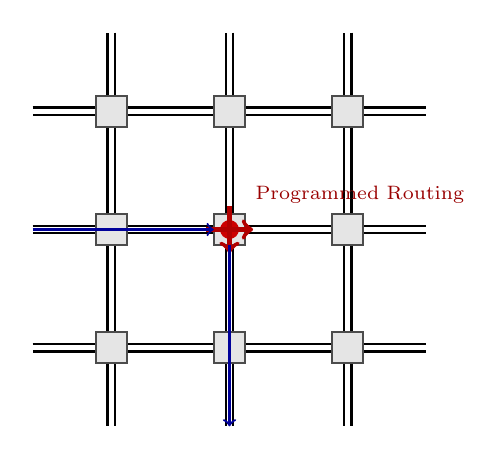
\begin{tikzpicture}[scale=1.0, thick]

  % -- FPGA Grid Lines (Rows) --
  \draw[double, double distance=2pt] (-2.5, 1.5) -- (2.5, 1.5);
  \draw[double, double distance=2pt] (-2.5, 0.0) -- (2.5, 0.0);
  \draw[double, double distance=2pt] (-2.5, -1.5) -- (2.5, -1.5);

  % -- FPGA Grid Lines (Columns) --
  \draw[double, double distance=2pt] (-1.5, 2.5) -- (-1.5, -2.5);
  \draw[double, double distance=2pt] (0.0, 2.5) -- (0.0, -2.5);
  \draw[double, double distance=2pt] (1.5, 2.5) -- (1.5, -2.5);

  % -- Crossover Nodes (Active Routing) --
  \foreach \x in {-1.5, 0.0, 1.5} {
    \foreach \y in {-1.5, 0.0, 1.5} {
      \fill[gray!20] (\x-0.2, \y-0.2) rectangle (\x+0.2, \y+0.2);
      \draw[gray!60!black] (\x-0.2, \y-0.2) rectangle (\x+0.2, \y+0.2);
    }
  }

  % -- Specifically active triode node --
  \fill[red!80!black] (0, 0) circle (0.12);
  \draw[->, red!70!black, ultra thick] (-0.3, 0) -- (0.3, 0);
  \draw[->, red!70!black, ultra thick] (0, 0.3) -- (0, -0.3);
  \node[above right, font=\scriptsize, red!60!black] at (0.2, 0.2) {Programmed Routing};

  % -- Flow tracking --
  \draw[->, thick, blue!60!black] (-2.5, 0) -- (-0.2, 0);
  \draw[->, thick, blue!60!black] (0, -0.2) -- (0, -2.5);
  
\end{tikzpicture}
\caption{\textbf{Continuous FPGA Matrix.} A crossbar array of intersecting waveguides. At every matrix crossover point lies an embedded programmable Geometric Triode router. By asserting static topological strain masks to specific intersections (red dot / arrows), traveling data waves (blue arrows) are dynamically blocked or deflected through the native spatial fabric.}
\label{fig:sym_fpga}
\end{figure}

\noindent\textit{EE Equivalent:} FPGA lookup table fabric / Crossbar switch. \quad\textit{Key Physics:} Matrix-level spatial routing logic.

%% ============================================================
%% 19. HOLOGRAPHIC SOLITON ARRAY
%% ============================================================
\subsection{Holographic Soliton Array (Macro Memory)}
\label{sym:holographic_array}

\begin{figure}[ht]
\centering
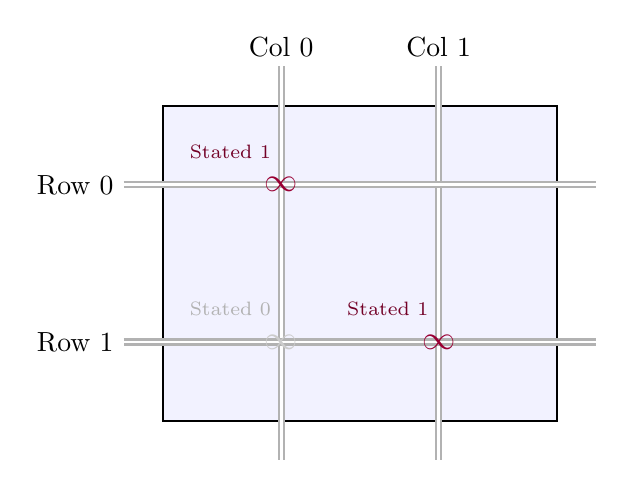
\begin{tikzpicture}[scale=1.0, thick]

  % -- 2D Matrix Plane --
  \draw[fill=blue!5, draw=black] (-2.5, -2.0) rectangle (2.5, 2.0);

  % -- Vertical Drive Lines (Cols) --
  \draw[double, double distance=1pt, gray!60] (-1.0, 2.5) -- (-1.0, -2.5);
  \draw[double, double distance=1pt, gray!60] (1.0, 2.5) -- (1.0, -2.5);

  % -- Horizontal Drive Lines (Rows) --
  \draw[double, double distance=1pt, gray!60] (-3.0, 1.0) -- (3.0, 1.0);
  \draw[double, double distance=1pt, gray!60] (-3.0, -1.0) -- (3.0, -1.0);

  % -- Soliton Knots --
  \node[font=\large, purple!80!black] at (-1.0, 1.0) {$\infty$};
  \node[font=\large, purple!80!black] at (1.0, -1.0) {$\infty$};
  \node[font=\large, gray!40] at (-1.0, -1.0) {$\infty$}; % Empty (Q=0 state represented faintly)

  % -- Labels --
  \node[above left, font=\scriptsize, purple!60!black] at (-1.0, 1.2) {Stated 1};
  \node[above left, font=\scriptsize, purple!60!black] at (1.0, -0.8) {Stated 1};
  \node[above left, font=\scriptsize, gray!60] at (-1.0, -0.8) {Stated 0};

  % -- Row/Col Labels --
  \node[left] at (-3.0, 1.0) {Row 0};
  \node[left] at (-3.0, -1.0) {Row 1};
  \node[above] at (-1.0, 2.5) {Col 0};
  \node[above] at (1.0, 2.5) {Col 1};

\end{tikzpicture}
\caption{\textbf{Holographic Soliton Array.} The macro-level organization of non-volatile topological memory. Instead of discrete physical memory cell transistors, the array is a continuous 2D vacuum plane bounded by write/read waveguides. Soliton kinks ($\infty$, $Q=1$) localize seamlessly at waveguide intersections when $\Phi_{pack}\,V_{snap}$ amplitude is coincidentally reached by Row+Column wavefronts.}
\label{fig:sym_holographic_array}
\end{figure}

\noindent\textit{EE Equivalent:} Cross-Point Memory / 3D NAND matrix. \quad\textit{Key Physics:} 2D spatial superposition $V_{total} = V_{row} + V_{col}$.
